\documentclass[titlepage]{article}
\usepackage{babel}
\usepackage{amsmath}
\usepackage{amssymb}
\usepackage{amsthm}
\usepackage{tabto} %tabulator mit \tab
\usepackage{tikz}
\usetikzlibrary{automata, arrows.meta, positioning, shadows, shapes.geometric} % automaten zeichnen
\usepackage[utf8]{inputenc}
\pagestyle{plain}
\pagenumbering{arabic}
\renewcommand{\arraystretch}{1.3} %vertikaler abstand von tabellen
\usepackage[left=20mm, right=15mm, top=25mm, bottom=7mm, paper=a4paper]{geometry}

\renewcommand{\contentsname}{Inhaltsverzeichnis}
\renewcommand{\]}{\right]}
\renewcommand{\[}{\left[}
\renewcommand{\)}{\right)}
\renewcommand{\(}{\left(}
\renewcommand{\|}{\;|\;}
\newcommand{\n}{\newline}
\renewcommand{\l}{\linebreak}



\begin{document}\begingroup\let\clearpage\relax
	%header
	\begin{center}
	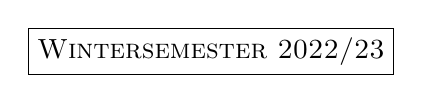
\begin{tikzpicture}
		\draw (0,0) node[draw, rectangle]{\textsc{Wintersemester 2022/23}};
	\end{tikzpicture}
	\hrulefill\\
	\begin{center}
		\LARGE\textsc{Automaten und Berechenbarkeit - Übung 04} \normalsize\\
	\end{center}
	\hrulefill
	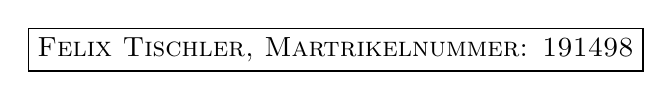
\begin{tikzpicture}
		\draw (0,0) node[draw, rectangle]{\textsc{Felix Tischler, Martrikelnummer: 191498}};
	\end{tikzpicture}
	\date{\today}
\end{center}
	
	%task one
	\section*{Aufgabe 1}
		\tab NFA $M=(\{0,1\},\{a,b,c,d\},\delta,\{a,d\},\{b,d\})$\tab$\delta$:\l
		\begin{center}
			\centering
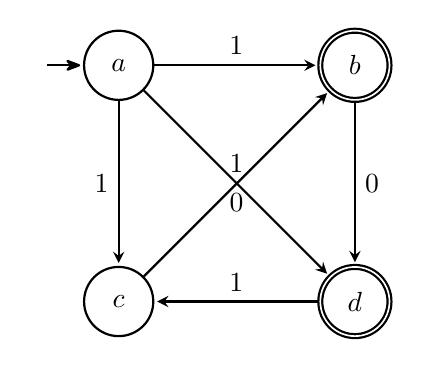
\begin{tikzpicture}[shorten >=1pt,node distance=3cm,on grid,>={Stealth[round]},thick]
	
	\node (a) [state, initial, initial text = {}] {$a$};
	\node (b) [state, accepting, right of = a] {$b$};
	\node (c) [state, below of = a] {$c$};
	\node (d) [state, accepting, right of = c] {$d$};
	
	\path [-stealth, thick]
	(a) edge node [above] {1} (b)
	(a) edge node [left] {1} (c)
	(a) edge node [above] {1} (d)
	(b) edge node [right] {0} (d)
	(c) edge node [below] {0} (b)
	(d) edge node [above] {1} (c);
	
\end{tikzpicture}
			\newcommand{\q[1]}{$\{q_{#1}\}$}
\newcommand{\qq[1]}{$q_{#1}$}
\newcommand{\nz[2]}{$#1_#2$}
\newcommand{\nm[1]}{$\{#1\}$}

\begin{table}[h]
	\centering
	\begin{tabular}{|c|c|c|}
		\hline
		Zustand & 0 & 1 \\
		\hline\hline
		$\emptyset$&$\emptyset$&$\emptyset$\\
		\hline
		a&$\emptyset$&\nm[b,c,d]\\
		\hline
		b&\nm[d]&$\emptyset$\\
		\hline
		c&\nm[b]&$\emptyset$\\
		\hline
		d&$\emptyset$&\nm[c]\\
		\hline
	\end{tabular}
\end{table}

		\end{center}
	
		\subsection*{(a)}
			
\begin{align*}
	\delta^*(\{a\},1001)&=\bigcup_{z\in\{a\}}(\delta(\{a\},1),001)\\
	&=\delta^*(\{b,c,d\},001)\\
	&=\bigcup_{z\in\{b,c,d\}}\delta^*(\delta(\{b,c,d\},0),01)\\
	&=\delta^*(\{d\},01)\cup\delta^*(\{b\},01)\cup\delta^*(\emptyset,01)\\
	&=\delta^*(\delta(\{d\},0),1)\cup\delta^*(\delta(\{b\},0),1)\\
	&=\emptyset\cup\delta^*(\{d\},1)\\
	&=\delta^*(\delta(\{d\},1),\lambda)\\
	&=\delta^*(\{c\},\lambda)\\
	&=\{c\}
\end{align*}

			
\begin{align*}
	\delta^*(\{d\},1000)&=\delta^*(\delta(\{d\},1),000)\\
	&=\delta^*(\{c\},000)\\
	&=\delta^*(\delta(\{c\},0),00)\\
	&=\delta^*(\{b\},00)\\
	&=\delta^*(\delta(\{b\},0),0)\\
	&=\delta^*(\{d\},0)\\
	&=\delta^*(\delta(\{d\},0),\lambda)\\
	&=\delta^*(\emptyset,\lambda)=\emptyset
\end{align*}

			
		\subsection*{(b)}Bestimmen Sie $\{w\in\{0,1\}^*\mid\delta^*(\{a\},w)\cap\{d\}\neq\emptyset\}!$
			
\begin{align*}
	\delta^*(\{a\},w)...\text{ Menge der möglichen Endzustände, in denen man landet, wenn man }w\text{ abgearbeitet hat.}
\end{align*}
Da $\delta^*({a},w)\cup\{d\}\neq\emptyset$ gelten soll, muss $d\in\delta^*({a},w)$. 1. Fall: direkt aus $a$ nach $d$. 2. Fall aus $a$ nach $b$ und dann nach $d$. 3. Fall aus $a$ nach $c$ und dann nach $d$. 4. Fall: einer der drei Fälle und dann aus $d$ nach $c$ und dann nach $b$ und dann wieder nach $d$. \\\\
Aus Fall 1 bis 4 ergeben sich folgende Muster in den akzeptierten Wörtern:
\begin{cases}
	1.\quad w=1=a\\
	2.\quad w=10=b\\
	3.\quad w=100=c\\
	4.\quad w=a100|b100|c100
\end{cases}\\\\\\
Der 4. Fall kann als einziger immer wieder angewandt werden ohne, dass die Akzeptanz von $w$ beeinflusst wird. Somit ergibt sich: $\{w\in\{0,1\}^*\mid\delta^*(\{a\},w)\cap\{d\}\neq\emptyset\}=\underline{\{1,10,100\}\cdot\{100\}^*}$
			
		\subsection*{(c)}
		Übergangstabelle des gegebenen NFA $M$:
		\begin{center}
			\newcommand{\q[1]}{$\{q_{#1}\}$}
\newcommand{\qq[1]}{$q_{#1}$}
\newcommand{\nz[2]}{$#1_#2$}
\newcommand{\nm[1]}{$\{#1\}$}

\begin{table}[h]
	\centering
	\begin{tabular}{|c|c|c|}
		\hline
		Zustand & 0 & 1 \\
		\hline\hline
		$\emptyset$&$\emptyset$&$\emptyset$\\
		\hline
		a&$\emptyset$&\nm[b,c,d]\\
		\hline
		b&\nm[d]&$\emptyset$\\
		\hline
		c&\nm[b]&$\emptyset$\\
		\hline
		d&$\emptyset$&\nm[c]\\
		\hline
		\nm[b,c,d]&\nm[d,b]&\nm[c]\\
		\hline
		\nm[d,b]&\nm[d]&\nm[c]\\
		\hline
	\end{tabular}
	Bzw.
	\begin{tabular}{|c|c|c|}
		\hline
		Zustand & 0 & 1 \\
		\hline\hline
		$\emptyset$&$\emptyset$&$\emptyset$\\
		\hline
		\qq[0]&$\emptyset$&\q[4]\\
		\hline
		\qq[1]&\q[3]&$\emptyset$\\
		\hline
		\qq[2]&\q[1]&$\emptyset$\\
		\hline
		\qq[3]&$\emptyset$&\q[2]\\
		\hline
		\qq[4]&\q[5]&\q[2]\\
		\hline
		\qq[5]&\q[3]&\q[2]\\
		\hline
	\end{tabular}	
\end{table}

		\end{center}
		Bestimmung der Einträge in der Übergangstabelle:
		\begin{center}	
			\begin{math}
	\delta^*(\{d,b\},0)=
	
	\delta^*(\{d,b\},1)=
	
	\delta^*(\{b,c,d\},0)=
	
	\delta^*(\{b,c,d\},1)=
\end{math}
		\end{center}
		DFA $M'$:
		\begin{center}
			$\delta^{'}$:\l
			\centering
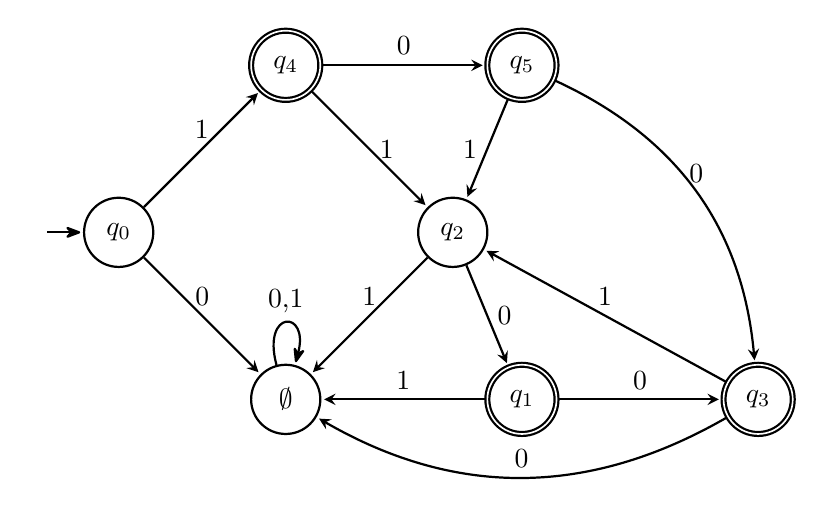
\begin{tikzpicture}[shorten >=1pt,node distance=3cm,on grid,>={Stealth[round]},thick]
	
	\node (q0) [state, initial, initial text = {}] {$q_0$};
	\node (q4) [state, accepting, above right of = q0] {$q_4$};
	\node (empty) [state, below right of = q0] {$\emptyset$};
	\node (q1) [state, accepting, right of = empty] {$q_1$};
	\node (q2) [state, below right of = q4] {$q_2$};
	\node (q3) [state, accepting, right of = q1] {$q_3$};
	
	\node (q5) [state, accepting, right of = q4] {$q_5$};
	
	\path [-stealth, thick]
	(empty) edge [loop above] node {0,1} (empty)
	(q0) edge node [above] {0} (empty)
	(q0) edge node [above] {1} (q4)
	
	(q1) edge node [above] {0} (q3)
	(q1) edge node [above] {1} (empty)
	
	(q2) edge node [right] {0} (q1)
	(q2) edge node[above] {1} (empty)
	
	(q3) edge [bend left] node [above] {0} (empty)
	(q3) edge node [above] {1} (q2)
	
	(q4) edge node [above] {0} (q5)
	(q4) edge node [right] {1} (q2)
	
	(q5) edge [bend left] node [above] {0} (q3)
	(q5) edge node [left] {1} (q2);
\end{tikzpicture}\l
			$M^{'}=(\{0,1\},Z',\delta',S',Z_E')$
		\end{center}
	\section*{Aufgabe 2}
	\subsection*{(a)}
		Der DFA ist mittel Potenzmengenkonstruktion aus dem NFA in (b) entstanden. Die Zustände $z_2$ und $z_3$ wurden entfernt, da Sie nicht erreichbar sind. Im Teil (b) habe ich den NFA bewiesen. Da dieser DFA auf jenem beruht gilt er ebenso.\\\\
		\tab$M'=(\{0,1\},Z',\delta^{'},S',Z_E')$\tab$\delta$:\\
		\begin{center}
			\centering
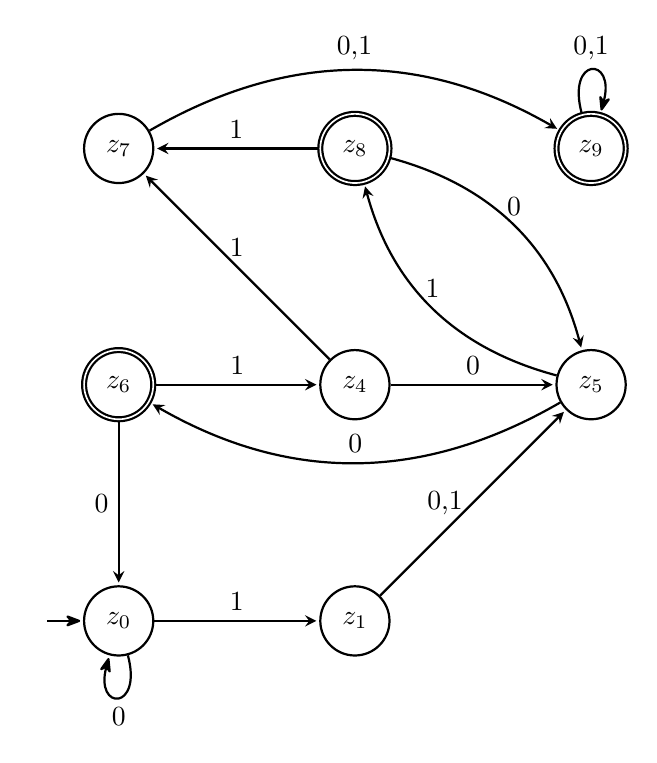
\begin{tikzpicture}[shorten >=1pt,node distance=3cm,on grid,>={Stealth[round]},thick]
	
	\node (z0) [state, initial, initial text = {}] {$z_0$};
	\node (z1) [state, right of = z0] {$z_1$};
	%\node (z2) [state, below of = z1] {$z_2$};
	%\node (z3) [accepting, state, right of = z2] {$z_3$};
	\node (z4) [state, above of = z1] {$z_4$};
	\node (z5) [state, right of = z4] {$z_5$};
	\node (z6) [accepting, state, above of = z0] {$z_6$};
	\node (z7) [state, above of = z6] {$z_7$};
	\node (z8) [accepting, state, right of = z7] {$z_8$};
	\node (z9) [accepting, state, right of = z8] {$z_9$};
	
	\path [-stealth, thick]
	(z0) edge [loop below] node {0} (z0)
	(z0) edge node [above] {1} (z1)
	
	(z1) edge node [left] {0,1} (z5)
	
	%(z2) edge [bend left] node [above] {0,1} (z6)
	
	%(z3) edge [bend left] node [above] {0,1} (z0)

	(z4) edge node [above] {0} (z5)
	(z4) edge node [above] {1} (z7)
	
	(z5) edge [bend left] node [above] {0} (z6)
	(z5) edge [bend left] node [above] {1} (z8)
	
	(z6) edge node [left] {0} (z0)
	(z6) edge node [above] {1} (z4)
	
	(z7) edge [bend left] node [above] {0,1} (z9)
	
	(z8) edge [bend left] node [above] {0} (z5)
	(z8) edge node [above] {1} (z7)
	
	(z9) edge [loop above] node [above] {0,1} (z9);

	

\end{tikzpicture}
			\newcommand{\z[1]}{$\{z_{#1}\}$}
\newcommand{\zz[1]}{$z_{#1}$}
\newcommand{\nz[2]}{$#1_#2$}
\newcommand{\nm[1]}{$\{#1\}$}

\begin{table}[h]
	\centering
	\begin{tabular}{|c|c|c|}
		\hline
		Zustand & 0 & 1 \\
		\hline\hline
		\zz[0]&\z[0]&\z[1]\\
		\hline
		\zz[1]&\nm[z_0,z_2]&\nm[z_0,z_2]\\
		\hline
		\zz[2]&\nm[z_0,z_3]&\nm[z_0,z_3]\\
		\hline
		\zz[3]&\z[0]&\z[0]\\
		\hline
		\nm[z_0,z_1]&\nm[z_0,z_2]&\nm[z_0,z_1,z_2]\\
		\hline
		\nm[z_0,z_2]&\nm[z_0,z_3]&\nm[z_0,z_1,z_3]\\
		\hline
		\nm[z_0,z_3]&\nm[z_0]&\nm[z_0,z_1]\\
		\hline
		\nm[z_0,z_1,z_2]&\nm[z_0,z_1,z_2,z_3]&\nm[z_0,z_1,z_2,z_3]\\
		\hline
		\nm[z_0,z_1,z_3]&\nm[z_0,z_2]&\nm[ z_0, z_1,z_2]\\
		\hline
		\nm[z_0,z_1,z_2,z_3]&\nm[ z_0,z_1,z_2,z_3]&\nm[z_0,z_1,z_2,z_3]\\
		\hline
	\end{tabular}
	Bzw.
	\begin{tabular}{|c|c|c|}
		\hline
		Zustand & 0 & 1 \\
		\hline\hline
		\zz[0]&\z[0]&\z[1]\\
		\hline
		\zz[1]&\nm[z_5]&\nm[z_5]\\
		\hline
		\zz[2]&\nm[z_6]&\nm[z_6]\\
		\hline
		\zz[3]&\z[0]&\z[0]\\
		\hline
		\zz[4]&\nm[z_5]&\nm[z_7]\\
		\hline
		\zz[5]&\nm[z_6]&\nm[z_8]\\
		\hline
		\zz[6]&\nm[z_0]&\nm[z_4]\\
		\hline
		\zz[7]&\nm[z_9]&\nm[z_9]\\
		\hline
		\zz[8]&\nm[z_5]&\nm[z_7]\\
		\hline
		\zz[9]&\nm[z_9]&\nm[z_9]\\
		\hline
	\end{tabular}
	
\end{table}
		\end{center}
	\subsection*{(b)}
		\tab$M=(\{0,1\},Z,\delta,S,Z_E)$\tab$\delta$:\\
		\begin{center}
			\centering
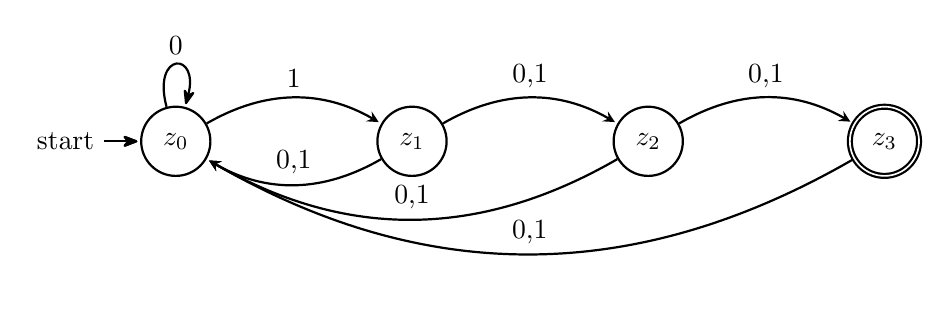
\begin{tikzpicture}[shorten >=1pt,node distance=3cm,on grid,>={Stealth[round]},thick]
	
	\node (z0) [state, initial, initial text = {}] {$z_0$};
	\node (z1) [state, right of = z0] {$z_1$};
	\node (z2) [state, right of = z1] {$z_2$};
	\node (z3) [state, right of = z2, accepting] {$z_3$};
	
	\path [-stealth, thick]
	(z0) edge [loop above, initial] node {0} (z0)
	(z0) edge [bend left] node [above] {1} (z1)
	
	(z1) edge [bend left] node [above] {0,1} (z2)
	(z1) edge [bend left] node [above] {0,1} (z0)
	
	(z2) edge [bend left] node [above] {0,1} (z3)
	(z2) edge [bend left] node [above] {0,1} (z0)
	
	(z3) edge [bend left] node [above] {0,1} (z0);
	
\end{tikzpicture}

			\newcommand{\z[1]}{$\{z_{#1}\}$}
\newcommand{\zz[1]}{$z_{#1}$}
\newcommand{\nz[2]}{$#1_#2$}
\newcommand{\nm[1]}{$\{#1\}$}

\begin{table}[h]
	\centering
	\begin{tabular}{|c|c|c|}
		\hline
		Zustand & 0 & 1 \\
		\hline\hline
		\zz[0]&\z[0]&\z[1]\\
		\hline
		\zz[1]&\nm[$z_0,z_2$]&\nm[$z_0,z_2$]\\
		\hline
		\zz[2]&\nm[$z_0,z_3$]&\nm[$z_0,z_3$]\\
		\hline
		\zz[3]&\z[0]&\z[0]\\
		\hline
	\end{tabular}
\end{table}
		\end{center}
		\begin{proof}[Beweis] $"\subseteq"$
	$\mid w\mid\ge3$ ist trivial. Wir sehen, dass der Automat frühestens nach einer Wortlänge von 3 ein Wort akzeptiert. Denn es muss mindestens $z_0\rightarrow z_1\rightarrow z_2\rightarrow z_3$ abgearbeitet sein um akzeptiert zu werden. Der Übergang von $z_0\rightarrow z_1$ bestimmt das 3. letzte Zeichen. Da $z_0\rightarrow z_1$ nur durch eine $1$ möglich ist, ist garantiert, dass das 3. letzte Zeichen eine 1 ist.
\end{proof}
\begin{proof}[Beweis] $"\supseteq"$
	Jedes Wort ist lesbar, da in jedem Zustand eine 0 oder 1 gelesen werden kann. Jedoch: kann ein Wort akzeptiert werden, so kann es nach beliebiger Anzahl von 0 und 1 in $z_0$ nach $z_1$ wandern, insofern der dritt letzte Buchstabe eine 1 ist (andern falls bleibt es in $z_0$). von dort kann es dann mit 2 variablen Buchstaben nach $z_3$ wo es schließlich akzeptiert wird. 
\end{proof}
	%task two
	
	\section*{Aufgabe 3}
	%task three
		\begin{center}
			\centering
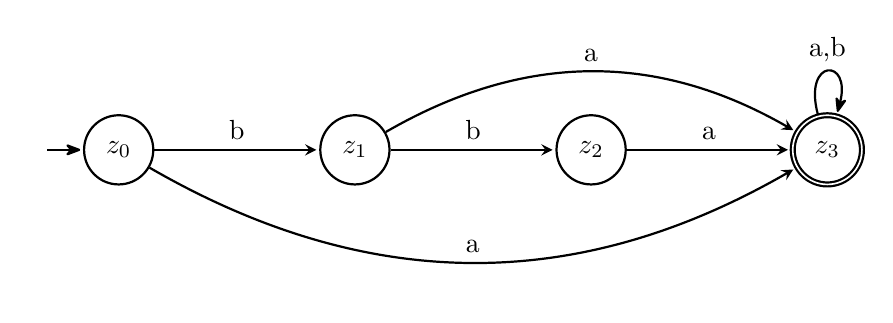
\begin{tikzpicture}[shorten >=1pt,node distance=3cm,on grid,>={Stealth[round]},thick]
	
	\node (z0) [state, initial, initial text = {}] {$z_0$};
	\node (z1) [state, right of = z0] {$z_1$};
	\node (z2) [state, right of = z1] {$z_2$};
	\node (z3) [state, right of = z2, accepting] {$z_3$};
	
	\path [-stealth, thick]
	(z0) edge [bend right] node [above] {a} (z3)
	(z0) edge node [above] {b} (z1)
	
	(z1) edge [bend left] node [above] {a} (z3)
	(z1) edge node [above] {b} (z2)
	
	(z2) edge node [above] {a} (z3)
	%(z2) edge [bend left] node [above] {b} (z0)
	
	(z3) edge [loop above] node {a,b} (z0);
	%(z3) edge [bend left] node [above] {b} (z0);
	
\end{tikzpicture}

			\newcommand{\q[1]}{$\{z_{#1}\}$}
\newcommand{\qq[1]}{$z_{#1}$}
\newcommand{\nz[2]}{$#1_#2$}
\newcommand{\qr[1]}{$#1$}
\newcommand{\nm[1]}{$\{#1\}$}
\newcommand{\row[4]}{\qq[#2]&\qq[#3]&\qq[#4]\\\hline}

\begin{table}[h]
	\centering
	\begin{tabular}{|c|c|c|}
		\hline
		Zustand & a & b \\
		\hline\hline
		\row{0}{3}{1}
		\row{1}{3}{2}
		\qq[2]&\qq[3]&$\emptyset$\\\hline
		\row{3}{3}{3}
	\end{tabular}
\end{table}

			\begin{proof}[Beweis] $"\subseteq"$
\end{proof}
\begin{proof}[Beweis] $"\supseteq"$
\end{proof}
		\end{center}
	
	\section*{Aufgabe 4}
	%task four
		\begin{center}
			\centering
\newcommand{\mynode[4]}{\node (#2) [#3] {#4};}
\renewcommand{\|}{\;|\;}
\begin{align*}
	G_1=(\{a,b\},\{S,A,B,E1,E2\},S,R)
	\text{ mit }R:
	\begin{cases}
		S&\rightarrow aA\|Bb\\
		A&\rightarrow E_1b\|b\\
		B&\rightarrow aE_2\|a\\
		E_1&\rightarrow aA\\\
		E_2&\rightarrow Bb
	\end{cases}
\end{align*}
\begin{proof}[Beweis] $"\subseteq"$
\end{proof}
\begin{proof}[Beweis] $"\supseteq"$
\end{proof}

		\end{center}

	\endgroup	
\end{document}